\renewcommand{\thesection}{\Roman{section}}
\section{Results}
\subsection*{Sensor Data}
The output data of the various sensors may indicate different modalities of the object being grasped. While the force torque sensor will react strongly to the weight of the object, the finger joint positions are more sensitive to the shape. Orthogonal to either of these, the tactile pressure sensors will give information of the object's compliance.

If we had obtained finger torque measurements, these would have additionally contributed to our picture of both the shape and the compliance of the object. Unfortunately, the data recording of the finger strain gages caused major technical difficulties so that it could not be done consistently. This was a severe setback, as the finger torques are the most sensitive measure to initial contact with the object. Not only did this halt our plans for a grasp preshaping algorithm, it also forced us to reprogram part of our data collection method.

Still, the remaining sensors give us quite a full and diverse description of an object. Let us discuss the finger positions. Figure \ref{fingerPos} shows the joint position profile while grasping the cone under each of the respective grasp types. The positional change is recorded in radians over the time span of the grasp. If we examine these graphs we can gain insight into the nature of both the grip and the object being grip.

Once the grasp is initiated, the position of each joint increases steadily until the object is fully enclosed in the hand. The joints remain at this maximal position until the object is released. The most interesting grip in this scenario is the top-down prismatic, where the hand grips the rather thin top of the cone. As the physical gap between fingers 1 and 2 is larger than the upper circumference of the cone, we can see that finger 1 fails to make full contact and thus moves further than finger 2. As opposed to this, in the side-on grips the fingers just wrap around the base of the cone, thereby only showing small positional variations. These differing scenarios play themselves out clearly in the sensor data. 
\begin{figure}[H]
        \centering
        \begin{subfigure}{0.5\textwidth}
                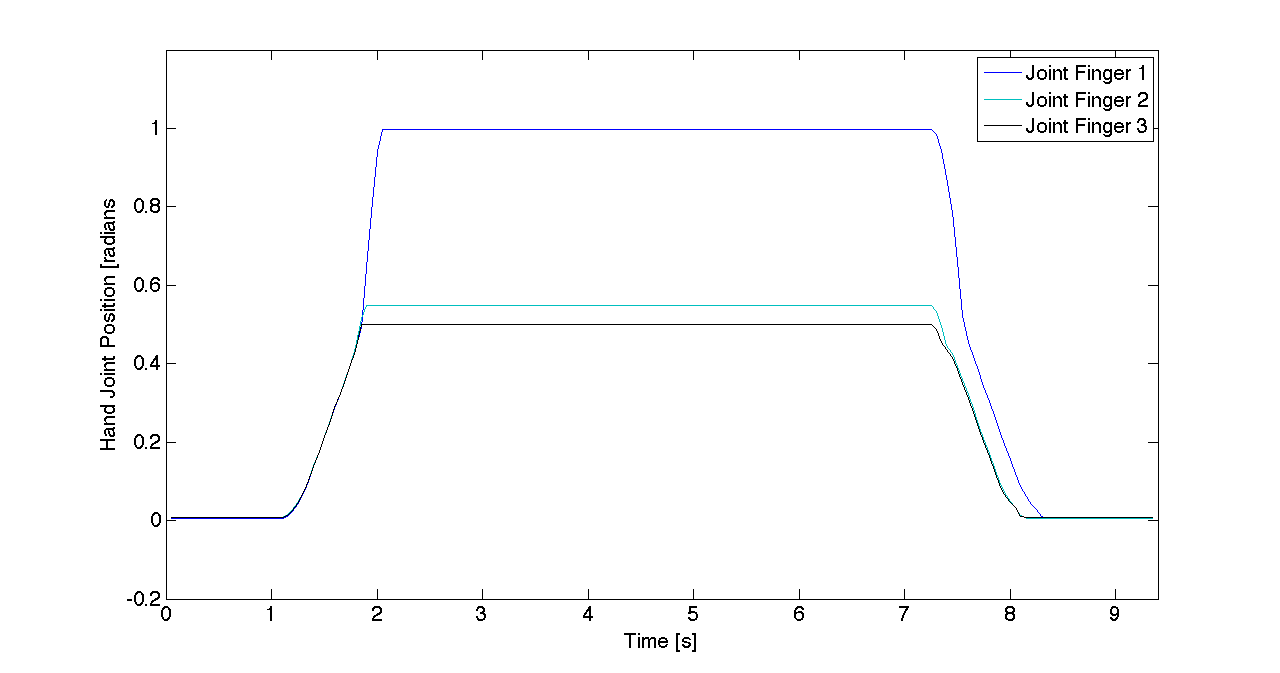
\includegraphics[width=\textwidth]{figFingerposM.png}
                \caption{Top-down Prismatic Precision}
        \end{subfigure}
        \begin{subfigure}{0.5\textwidth}
                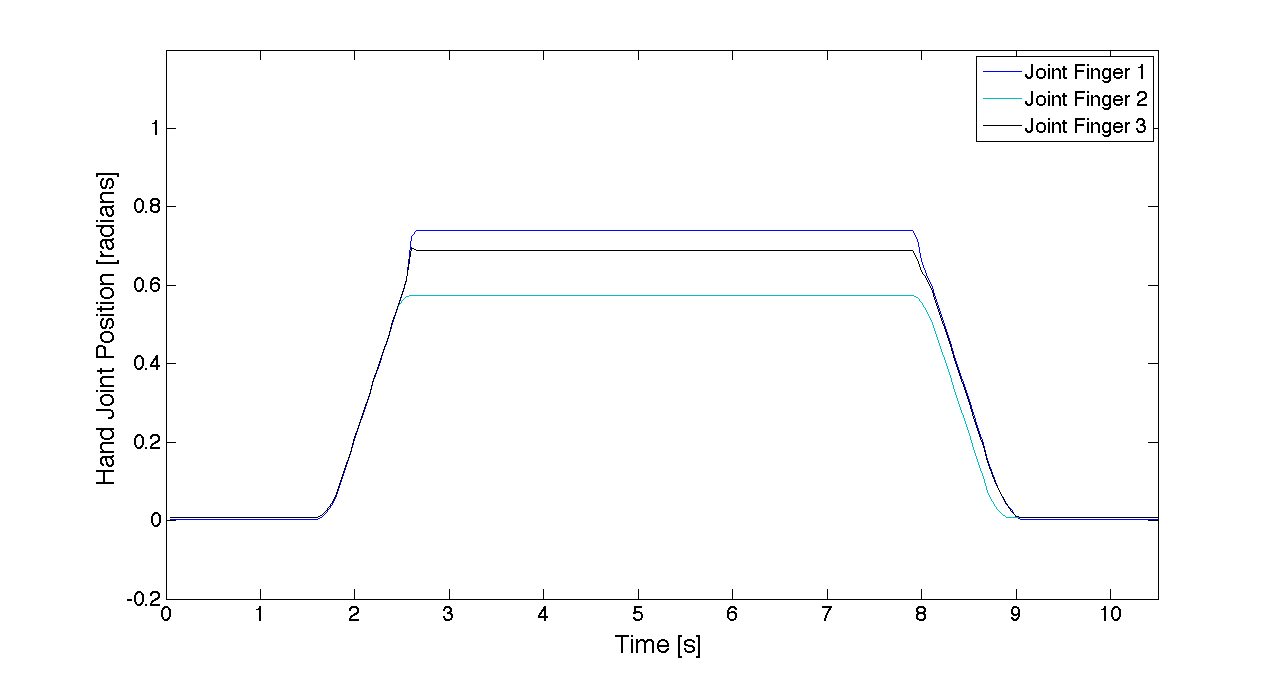
\includegraphics[width=\textwidth]{figFingerposW.png}
                \caption{Side-on Heavy Wrap}
        \end{subfigure}
        \begin{subfigure}{0.5\textwidth}
                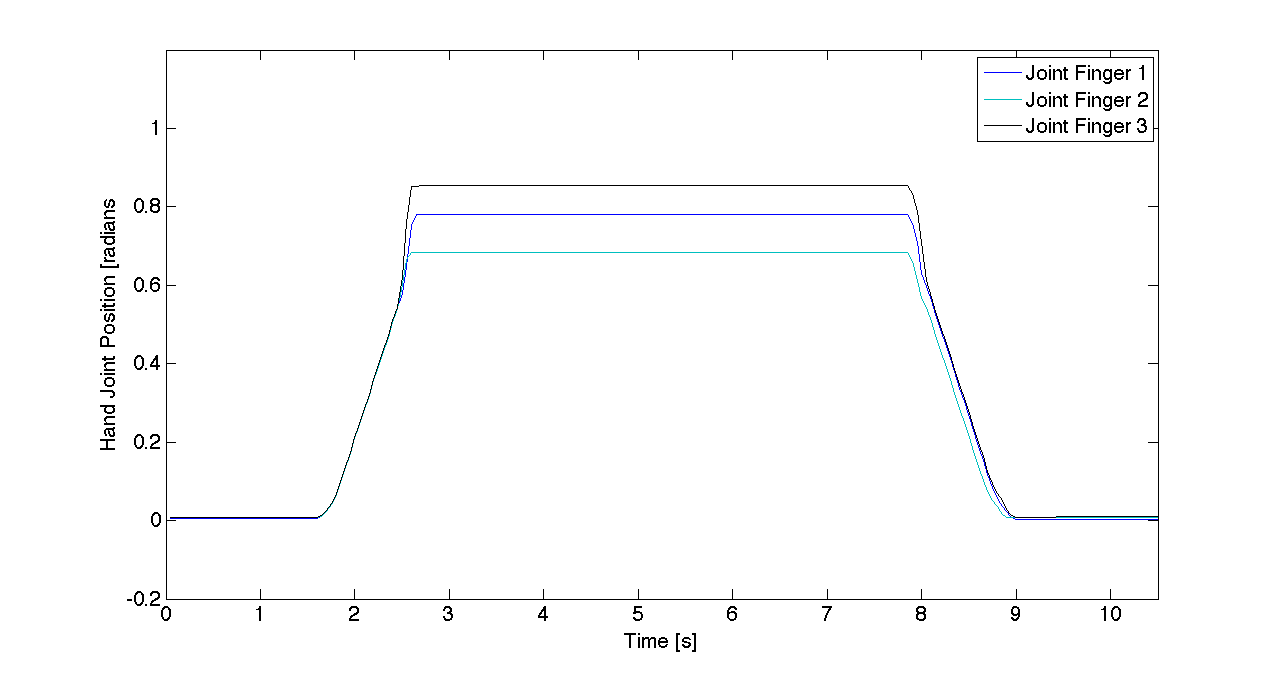
\includegraphics[width=\textwidth]{figFingerposG.png}
                \caption{Side-on Power Grip}
        \end{subfigure}
        \caption{Finger joint position in radians versus time for the (a) Prismatic Precision Grasp, the (b) Heavy Wrap, and the (c) Power Grip.}
        \label{fingerPos}
\end{figure}

We were especially interested in the output of the tactile pressure sensors. The three Barrett fingers as well as the palm are provided with a tactile sensor array, consisting of 24 pressure sensors. The sensors are arranged in an 8x3 array. In the following, the sensor cell will be referenced according to the enumeration given in figure \ref{senspos}. Note: the distal finger tip is always depicted at the top of the map, while the bottom cells represent the proximal end of the finger tip.
\begin{figure}[H]
        \centering
         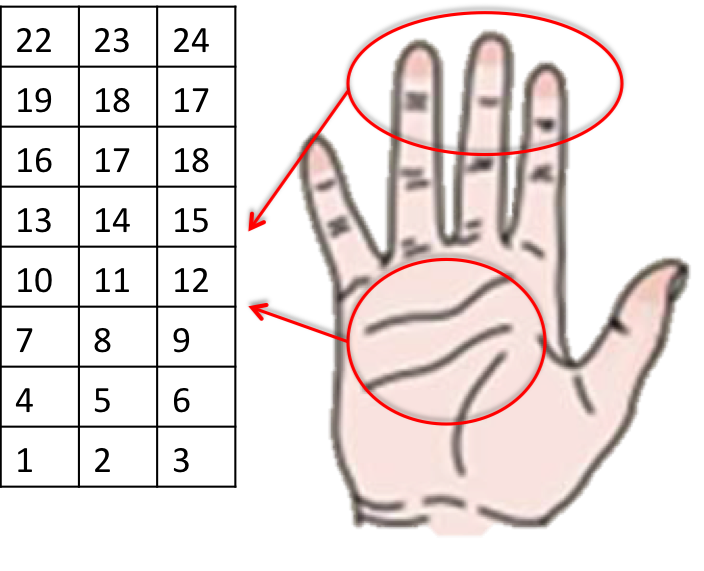
\includegraphics[width=0.3\textwidth]{sensor.png}
          \caption{Sensor arrays in finger tips and palm with 24 sensors each.}
          \label{senspos}
\end{figure}
\vspace{-0.25cm}
For each cell the mean pressure value during grasping was calculated for the respective finger/palm. We then compared different characteristics of the material to see which showed the most prominent feature in the pressure maps. Pressure values were recorded in $\frac{N}{cm^2}$. First, we compared the object's shape. Figure \ref{WoodvsBottle} shows two objects of similar weight: an upright square wood block (object 5) and a round water bottle (object 14 ), gripped with the Heavy Wrap.

The first observation is that for both objects, cells 1 and 4 in finger 1 show significantly higher pressures than all other cells. This was consistent through all measurements, grips, and objects of that specific data collection. We therefore conclude that something was blocking/triggering these cells leading to faulty data output. Consequently, we did not use these cells to train the neural network. 
\begin{figure*}%[H]
        \begin{subfigure}{\textwidth}
        \hspace{-2cm}
                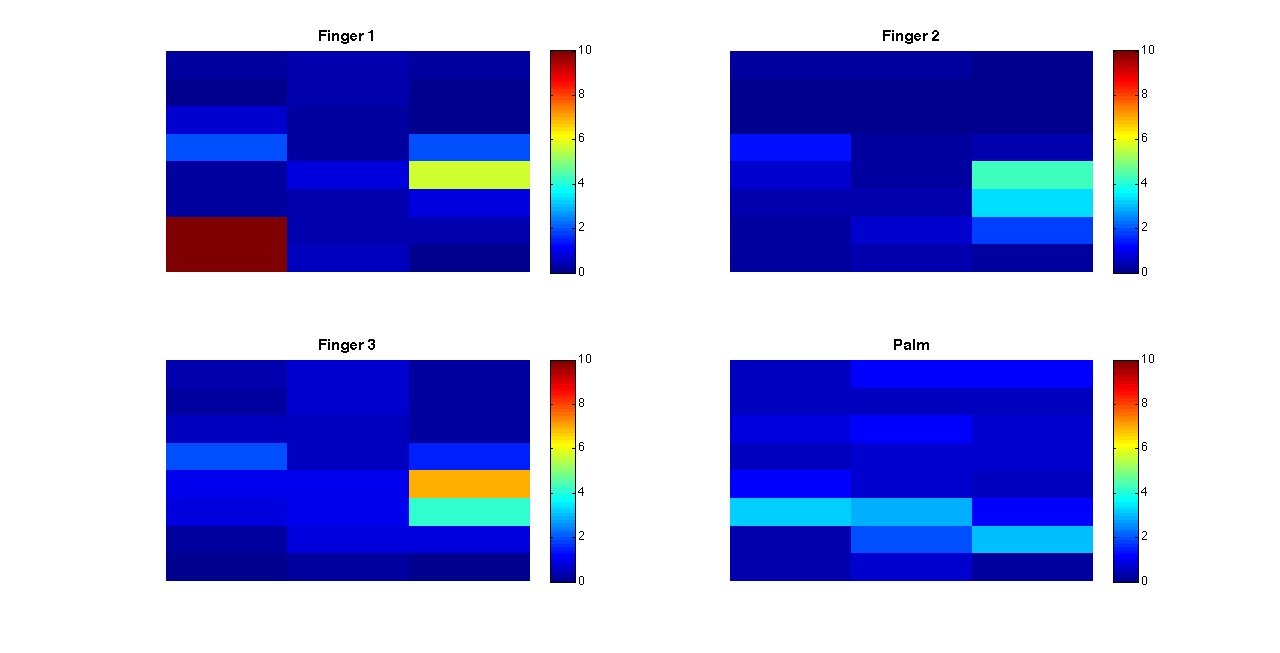
\includegraphics[width=1.2\textwidth]{figPressureWood.png}
                \vspace{-0.8cm}
                \caption{Side-on Heavy Wrap grip of square wood block (object 5)}
        \end{subfigure}\\[1cm]
        \begin{subfigure}{\textwidth}
        \hspace{-2cm}
                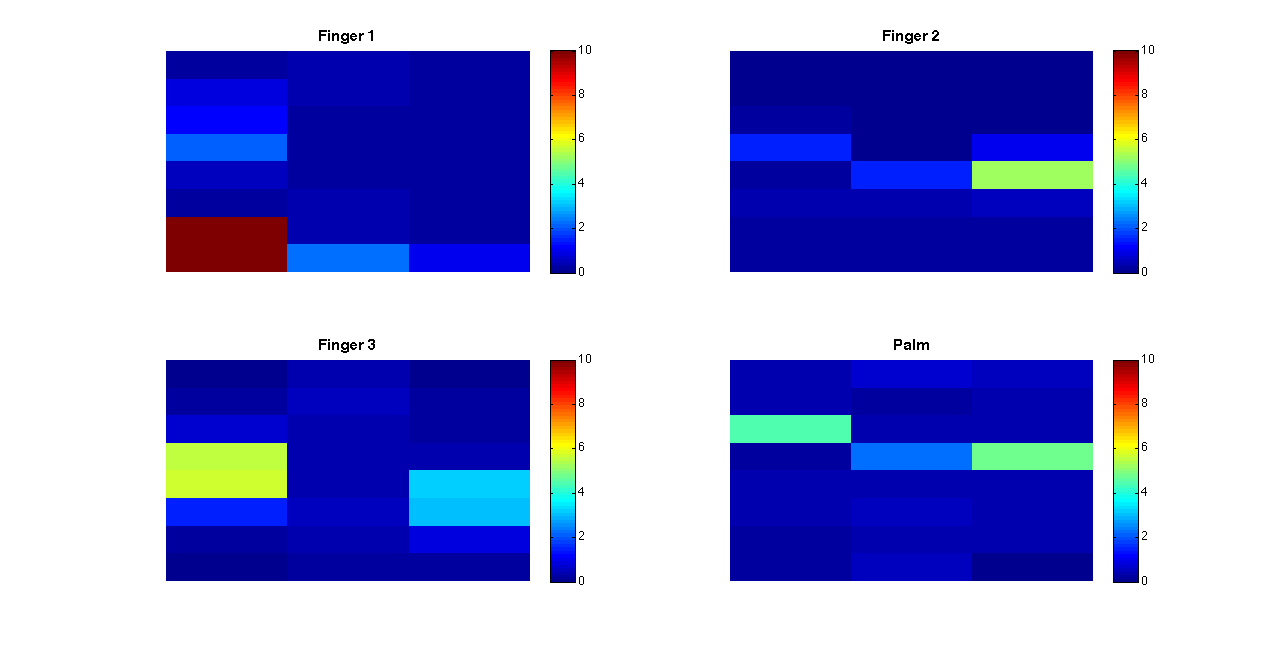
\includegraphics[width=1.2\textwidth]{figPressureBottle.png}
                \vspace{-0.8cm}
                \caption{Side-on Heavy Wrap grip of round water bottle (object 14)}
        \end{subfigure}
        \caption{Pressure maps of fingers 1-3 and palm of Barrett hand. Pressures are recorded in $\frac{N}{cm^2}$ and plotted as a mean over the grasping trial for each respective cells. The Side-on Heavy Wrap compared for a square and round object.}
        \label{WoodvsBottle}
\end{figure*}
\cleardoublepage
The pressure profiles differ slightly, mainly for the palm and for finger 1. As the object is being grasped from the side-on, the fingers wrap 
around it tightly. Accordingly, pressure sensors 7-18 are most prominent. Interestingly, the pressure is higher on the finger side than in the middle, which is most likely due to the bulky (rather square) shape of the Barrett Hand.

Even though the pressure maps show some distinctive features, the difference is not as striking as one might expect. However, unlike the human finger, the Barrett finger only has two phalanges, therefore it is not able to bend at the distal interphalangeal joint \cite{TortaGerardJ.2011}. The sensor array will therefore only touch one side of the wood log or the bottle, respectively, making it insensitive to the object's shape. 

Next, we compared the pressure profiles of two objects of the same shape, but different weight, surface structure, and slightly different size (compare figure \ref{WickervsStyro}). The two balls (rattan ball styrofoam ball) were gripped from top-down with the prismatic precision grasp. Again, sensors 1 and 4 showed faulty pressure data and were ignored. Unfortunately, sensor 3 of finger 1 also began to give unreasonable high feedback in the course of the data collection and was thus ignored. 

Again, the pressure maps show similar features. Most of the feedback is observed for the cells (7-18) in the middle of the finger. The pressure in J3 is slightly higher as finger 3 has to compensate for the two fingers (J1 and J2) gripping from the opposite site.  

It is interesting that the pressures while gripping the lighter styrofoam ball are slightly higher than the respective pressures while grasping the rattan ball. This is most likely due to the smaller size of the styrofoam ball. The fingers can consequently close further around the ball and thus tighten the grip. Additionally, the styrofoam ball has a smooth surface so that the fingers can tightly wrap around the surface, while the rattan ball has a rough surface that impede a tight grip.

The important factor of compliance becomes even more apparent, when comparing the pressure maps of a soft and hard piece of foam (compare figure \ref{SoftvsHard}) for a side-on power grip. The two objects, soft foam (object 2) as well as foam square (object4), were similar in size, shape, and weight. However, while the soft foam was very compliant, the foam square was rather firm. 

Note that again sensors 1 and 4 of finger 1 give faulty feedback and were not taken into account for any analysis. As the fingers approach side-on, they grab the square-shaped foam pieces longitudinally. The power grip really closed around the object until the foam was tightly squished. For the firm foam the two fingers push the square into an angled asymmetric position, so that the palm only receives pressure on one side, while J3 is pushing back hard with the distal end of the finger tip. As opposed to this, the pressure sensors show no response to the soft foam. This was consistent for all grasps of the soft foam and other soft objects, such as plush octopus (object 6). 

We conclude that the compliance of the object is the main factor which influences the response in the pressure sensors. The size of the object will influence how tightly it can be gripped and thus also show its effect, though indirectly. Grasping small objects such as the cube or the bean bag with the power grip, finger 1 will not make contact at all, thus leaving the pressure readout blank.

\begin{figure*}%[H]
        \begin{subfigure}{\textwidth}
        \hspace{-2cm}
                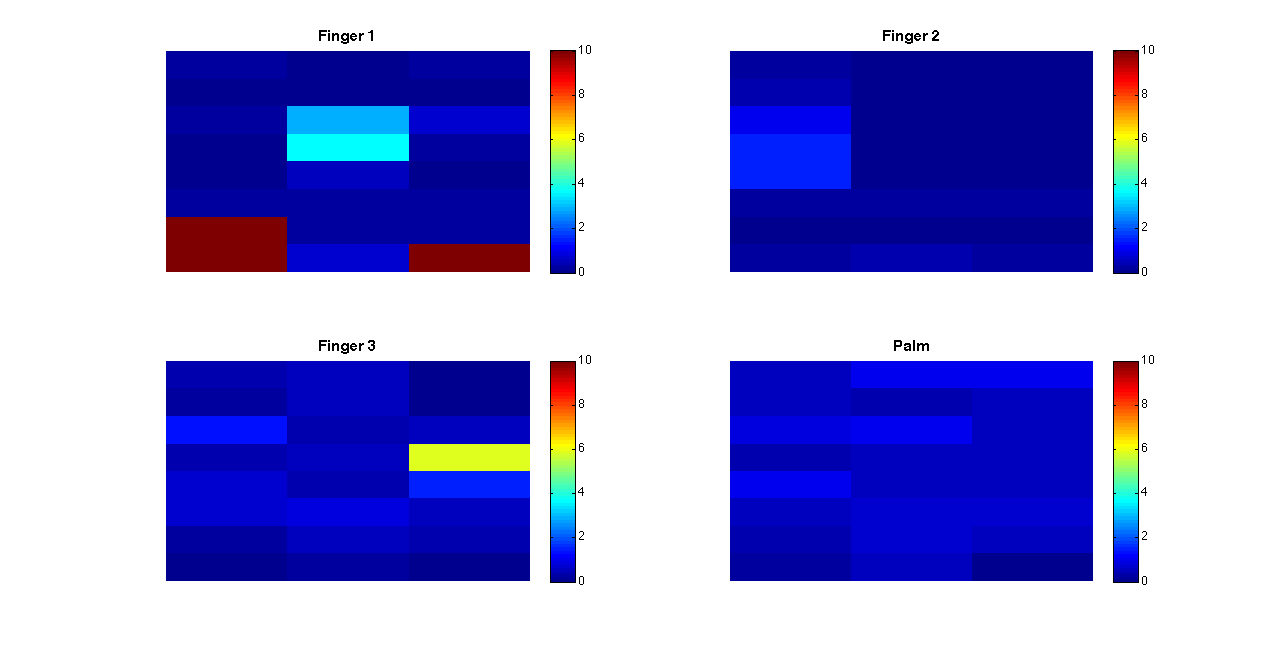
\includegraphics[width=1.2\textwidth]{figPressureWickerBall.png}
                \vspace{-0.8cm}
                \caption{Top-down Prismatic Precision grip of rattan ball (object 9)}
        \end{subfigure}\\[1cm]
        \begin{subfigure}{\textwidth}
        \hspace{-2cm}
                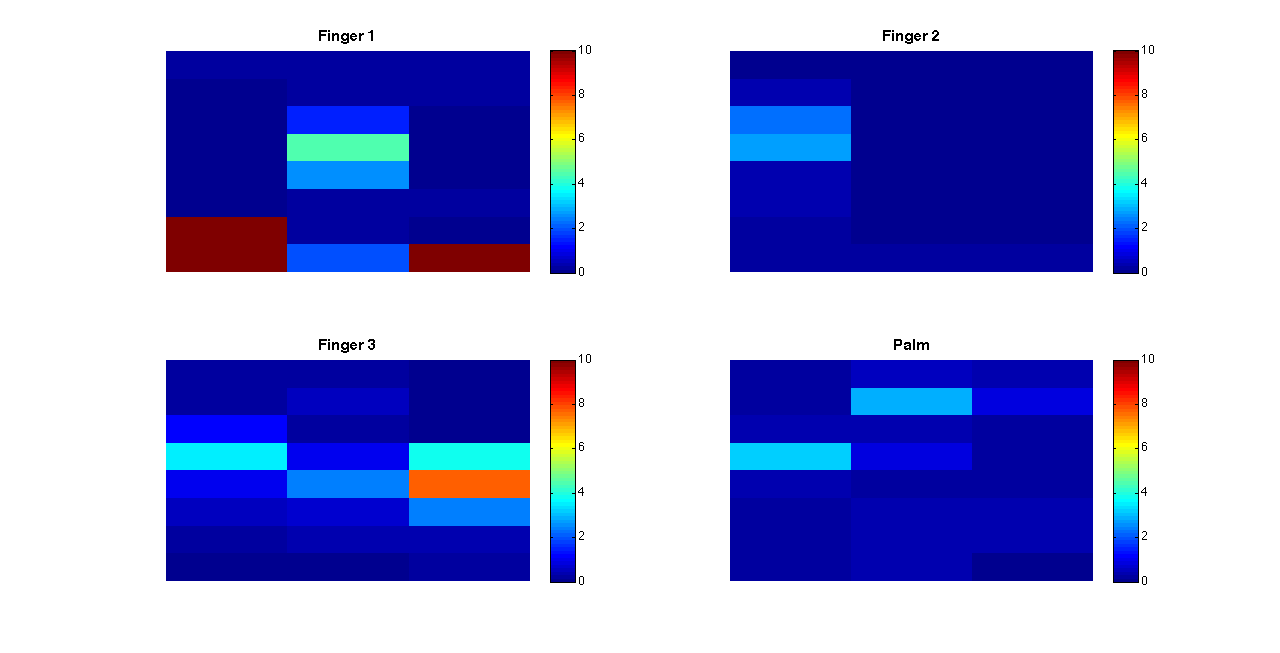
\includegraphics[width=1.2\textwidth]{figPressureBall.png}
                \vspace{-0.8cm}
                \caption{Top-down Prismatic Precision grip of styrofoam ball (object 1)}
        \end{subfigure}
        \caption{Pressure maps of fingers 1-3 and palm of Barrett Hand. Pressures are recorded in $\frac{N}{cm^2}$ and plotted as a mean over the grasping trial for each respective cells. The Top-down Prismatic Precision grip compared for two round objects with different weights and surface characteristics.}
        \label{WickervsStyro}
\end{figure*}
\cleardoublepage

\begin{figure*}%[H]
        \begin{subfigure}{\textwidth}
		\hspace{-2cm}
                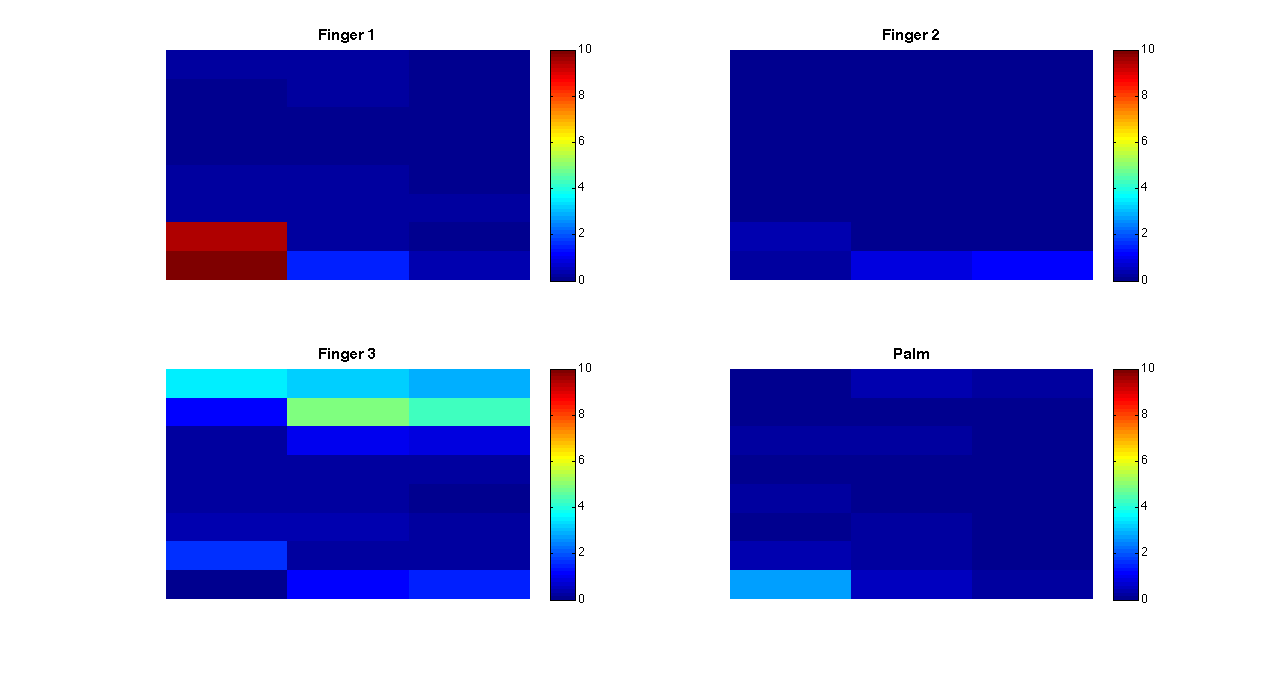
\includegraphics[width=1.2\textwidth]{figPressureHardSoft.png}
                \vspace{-0.8cm}
                \caption{Side-on Power Grip of hard foam square (object 4)}
        \end{subfigure}\\[1cm]
        \begin{subfigure}{\textwidth}
        \hspace{-2cm}
                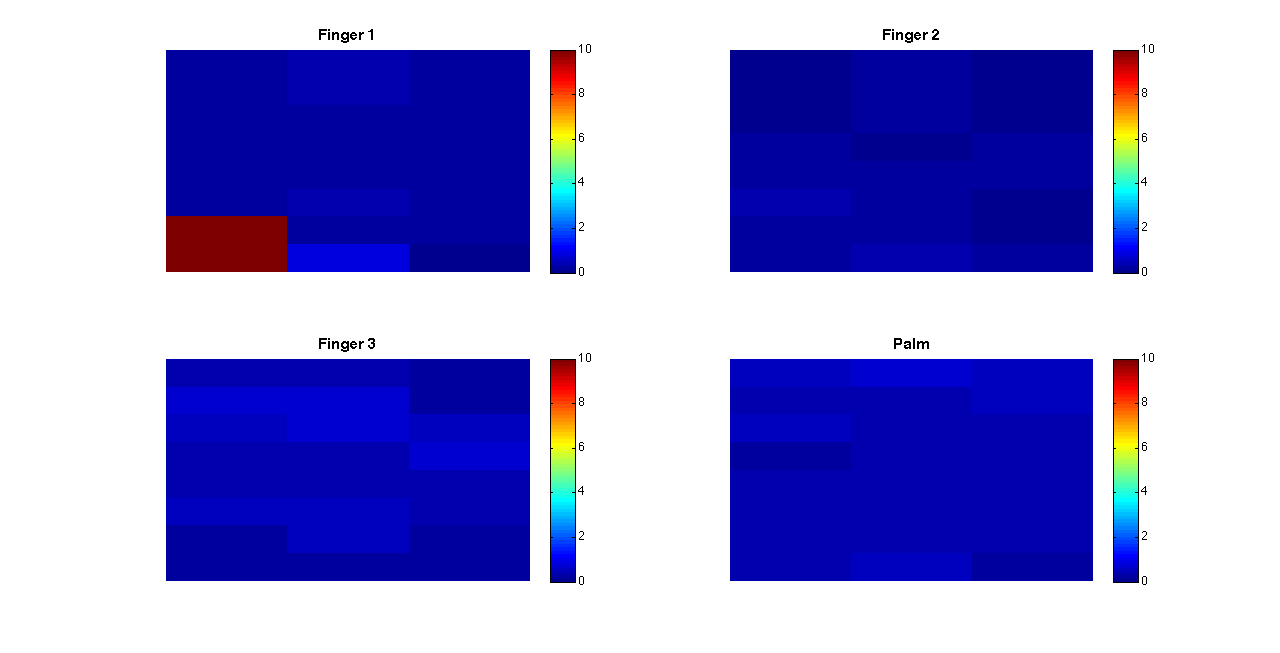
\includegraphics[width=1.2\textwidth]{figPressureSoftSoft.png}
                \vspace{-0.8cm}
                \caption{Side-on Power Grip of soft foam square (object 2)}
        \end{subfigure}
        \caption{Pressure maps of fingers 1-3 and palm of Barrett hand. Pressures are recorded in $\frac{N}{cm^2}$ and plotted as a mean over the grasping trial for each respective cells. The Side-on Power Grip compared for a soft and a hard square piece of foam.}
        \label{SoftvsHard}
\end{figure*}
\cleardoublepage

\subsection*{Neural Network}
The goal of the neural network analysis was to assign labels to certain objects and train the hand to familiarize itself with the sensor response generated by each object. In this way it should be able to recognize an object while grasping it, and then plan the next grasp accordingly. We tried to implement this method and improve its performance in the course of the project. Each step listed below was taken because the neural network analysis of the previous version showed no meaningful results (i.e. when performed on the robot it was not able to name an object correctly).
\begin{itemize}
\item Initially we attempted training on raw, unnormalized sensor data. The network performed poorly, attaining only 16\% accuracy even on the training set itself. We found that normalization of the data was absolutely crucial for training the neural network to good accuracy.
\item After normalization, the data set was split into training (80\%) and test data (20\%) randomly. For both training and validation the neural network analysis reached suspiciously high accuracy of more than 96\%. 
\item Faulty pressure readouts were detected and removed. We considered average read outs of over 15 $\frac{N}{cm^2}$ as faulty, especially when identical readings were observed over many different objects and grasp types.
\item The high accuracy on the test set and poor performance in the real world indicated to us that we had overfit the data. To mitigate this issue we increased the regularization weight. This led to a lower accuracy of training and validation step in the neural network analysis and seemed to favor certain objects for the respective grasp types. It did not significantly improve real-world performance, but did give us some insight to be discussed below.
\item As the number of trials for some objects were significantly higher than for others, we excluded these objects to provide a more balanced data set. This also seemed to afford no improvement.
\end{itemize}
Despite all our efforts to improve the neural network analysis, we were unable to obtain any kind of reliable performance. The fact that performance on the validation set nearly always matches performance on the training set \emph{should} indicate that no overfitting occurred. However, it may be the case that the validation data was in fact was too similar to the training data, since they were acquired as different time slices of the same grasp, rather than being taken from totally different grasp samples. This suspicion is emphasized by the 99\% accuracy of the neural network, a strong indication for overfitting the data.

Tests on the robot confirmed this. Objects could not be recognized correctly at all. However, for each grasp type, there were two or three select objects which would be identified correctly a majority of the time. The system seemed to prefer these objects and named these repeatedly, independent of which object was being grasped.

Adjusting the regularizer gave a lot of insight into this phenomenon. We were able to expose this behavior in the test data by using very heavy regularization. Running the network with $\lambda = 100$ led to a much lower accuracy for the neural network training---about 36\%. When we examined the individual predictions for each object, we found that there were a few objects which dominated. These objects were repeatedly predicted, thereby exhibiting 100\% recall (true positives\,/\,actual positives) but very low precision (true positives\,/\,predicted positives). The other objects therefore had 0\% recall.

To summarize, the neural network analysis did not work for the given training and validation data. It appears to be too heavily biased toward certain objects, though we are still unsure as to why. This behavior is usually not evident in the test set. Our conclusion is that either there were not enough individual grasps sampled, or the method does not hold for the desired task.